\documentclass[a4paper]{article}

\usepackage{graphicx}
\usepackage{amssymb}
\usepackage[utf8]{inputenc}
\usepackage[margin = 1in]{geometry}

\title{Física atómica: Litio}
\author{Iván Mauricio Burbano Aldana}

\begin{document}

\maketitle

En esta oportunidad se analizó el átomo de Litio mediante el método de Hartree. En este, a diferencia de todos los trabajos anteriores, el método se implementó en una hoja de cálculo LibreOffice Calc 5.1.6.2. Esto corresponde a que el código utilizado para el átomo de Helio demostró no ser lo suficientemente robusto frente a las dificultades de este nuevo calculo incluyendo:

\begin{itemize}

\item lo difícil que es mantener estable la solución de un nivel de energía bajo a radios altos;
\item ajustar las condiciones iniciales del potencial generado por cada electrón;
\item el acercamiento de diferentes niveles de energía para energías altas.

\end{itemize}

La hoja de cálculo permitió tener mucho más control sobre cada paso en la implementación pero hizo el proceso mucho más largo y sujeto a errores humanos. En las figuras \ref{fig:constantes}, \ref{fig:electron}, \ref{fig:potenciales} y \ref{fig:trabajo} se muestra la hoja utilizada. En particular, aprovechando la flexibilidad de las hojas de cálculo, en los niveles de energía $1s$ se realizaba la integración hasta el radio $30$. Despues de esto se asumía una función de onda nula. Además, es de notar que el cálculo de los potenciales se hizo de manera distinta. En la figura \ref{fig:electron} se puede observar que la integración del potencial generado por cada electrón se hizo desde afuera para adentro para asegurar que en el infinito el potencial fuera nulo. Finalmente, para diferenciar entre distintos niveles de energía se utilizaron las figuras generadas. La comparación con la forma de las funciones de onda del átomo de hidrógeno permitía identificar el estado del átomo.   

Las ecuaciones utilizadas se obtuvieron del enunciado de la tarea 7. Por lo tanto las unidades de las energías reportadas son de $E_0 = 122.4eV$ y las distancias de $a_0/3=1.76\times 10 ^{-11}m$. En las figuras \ref{fig:2s}, \ref{fig:2p}, \ref{fig:3s}, \ref{fig:3p} y \ref{fig:3d} se encuentran los resultados. En primer lugar, podemos notar que la forma de las funciones de onda y sus respectivas densidades de probabilidad siguen el modelo hidrogenoide. Esto refuerza la importancia del estudio del átomo de hidrógeno en la física atómica. En particular, el número de máximo de la distribución de probabilidad en un estado $(n,l)$ sigue cumpliendo la fórmula $n - (l-1)$. Vale la pena mencionar acá que los resultados en \ref{fig:3d} son anómalos. En particular la función de onda crece demasiado y no parece converger de manera suave a $0$. Esto se debe probablemente a que el rango de integración no es suficiente para describir el comportamiento de este estado. En segundo lugar, observamos que a medida que la energía del electrón exterior aumenta, la de los interiores disminuye y en general la del átomo disminuye. El comportamiento de los electrones interiores es de esperarse pues a medida que la energía del exterior aumenta este se aleja y disminuye su acción repulsiva sobre los otros. Sin embargo, el comportamiento de la energía total del átomo es inesperado. En efecto nuestros cálculos sugieren que los átomos se vuelven más estables a medida que el electrón exterior se aleja, lo cual no es correcto. Esto sugiere una impresición en el cálculo de las energías del electrón exterior que seguramente se debe al corte realizado en la integración de los átomos interiores. En efecto, ya que el valor esperado del electrón exterior está fuera del rango de integración de los electrones interiores, no se está teniendo en cuenta la totalidad del efecto repulsivo sobre él. En tercer lugar, podemos comparar las enegías calculadas con los encontrados en \cite{nist} para darnos una mejor idea sobre su precisión. Esta referencia pone en duda la precisión con la que se reportan los datos pues según ella la diferencia energética entre la configuración $1s^22s$ y $1s^22p$ debería ser cercana a $2eV$ mientras que los calculos no muestran ninguna diferencia. Así mismo, si bien la diferencia entre la configuración $1s^22p$ y $1s^23s$ no debería de ser de más de $2eV$ la diferencia calculada es de $8.9eV$. Sin embargo, podemos rescatar la similaridad entre las energías de las configuraciones $1s^23s$, $1s^23p$ y $1s^23d$.

Podemos concluir que el método utilizado fue exitoso para entender de manera cualitativa la distribución electrónica en el átomo de Litio y algunos detalles energéticos en los electrones interiores. Sin embargo, la falta de precisión en los cálculos y en particular en la integración del electrón exterior hizo difícil obtener conclusiones que reproduzcan la realidad de carácter cuantitativo. En particular, el método no hizo un buen trabajo en el cálculo de la energía total del átomo. Es importante notar que un gran factor en esto fue que el valor esperado de la posición del electrón exterior fue mayor al rango de integración de las funciónes de onda de los electrones interiores. Es necesario corregir este problema mejorando el método de integración utilizado. Creo que el entendimiento obtenido realizando las integraciones en la hoja de cálculo me ha dado la experiencia para afrontarme al reto de escribir un programa más robusto (en un lenguaje de menor nivel como C tal vez) que permita el cálculo más preciso de los niveles energéticos de este átomo. Finalmente, quiero recalcar que falta estudiar mejor los problemas de convergencia de las energías en el método de Hartree. Estos se pudieron observar en la tarea pasada con el átomo de Helio y fueron visibles cuando se intentó aplicar ese código al Litio. No fue posible estudiarlo en esta ocasión ya que para observar este fenómeno es necesario hacer en el orden de $30$ iteraciones, una tarea sencilla en un código pero muy difícil en las hojas de cálculo.

\begin{figure}
\begin{center}
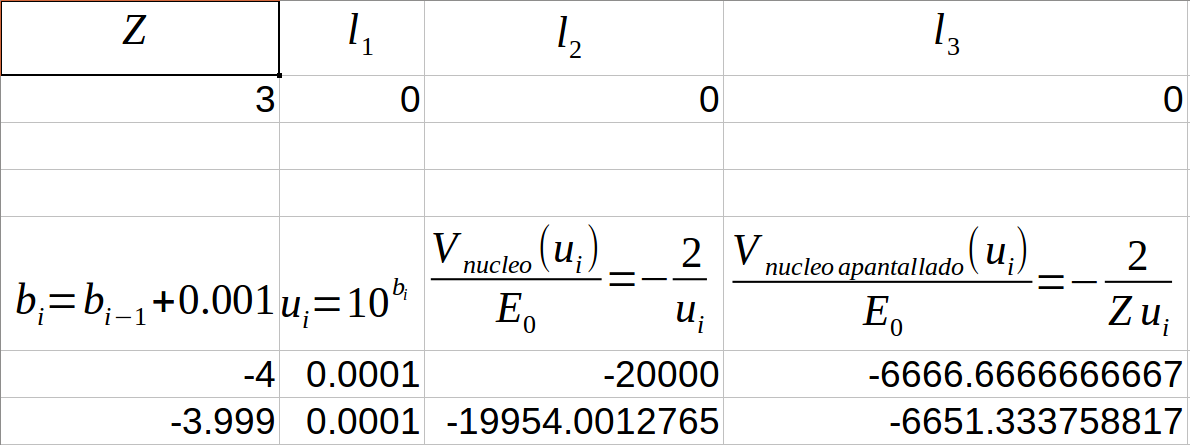
\includegraphics[width = 0.8\textwidth]{final_atomica_1.png}
\caption{\label{fig:constantes}Se utilizaron unas casillas para los valores del número cuántico orbital y se reservaron filas para la lista de posiciones y el potencial del nucleo. Notese que hasta el cálculo del estado $1s^2 2p$ se utilizó una escala de logarítmica de posiciones. Para los niveles más altos esta se dejó de utilizar en vista de que las funciones de onda calculadas ya no tenían la mayor parte de su actividad a valores bajos de radio.}
\end{center}
\end{figure}

\begin{figure}
\begin{center}
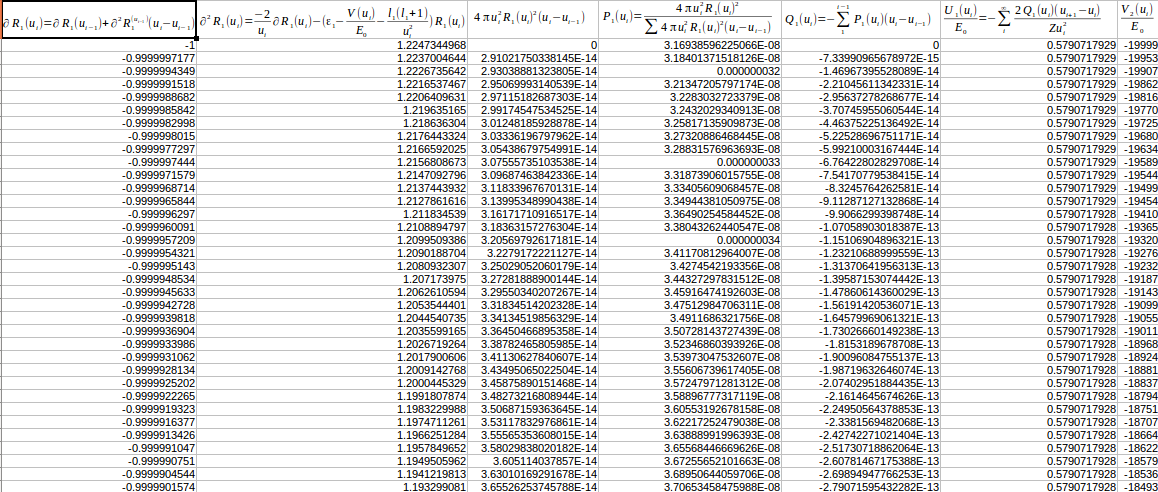
\includegraphics[width = \textwidth]{final_atomica_2.png}
\caption{\label{fig:electron}Se pusieron tres conjuntos de columnas como la que muestra en la figura. Cada una corresponde a un electrón y contiene toda su información relevante inclyendo su función de onda radial $R$ y el potencial que genera $U$. Las fórmulas utilizadas para calcular cada una de las columnas se encuentra en su título. La traducción a código es sencilla.}
\end{center}
\end{figure}

\begin{figure}
\begin{center}
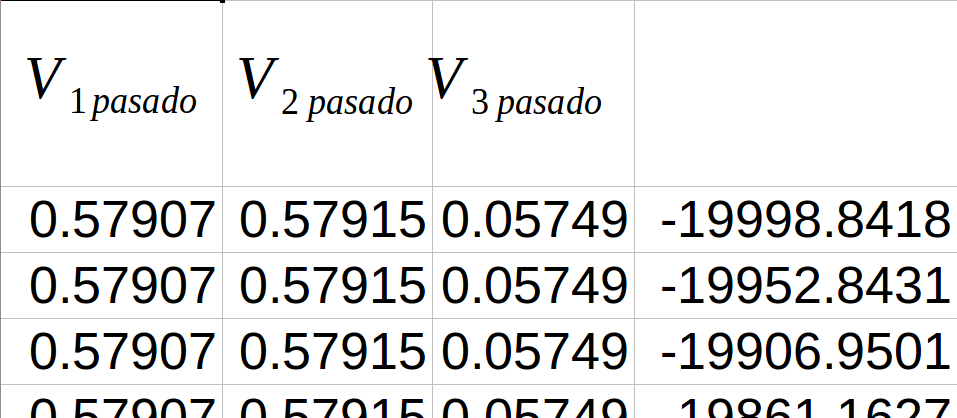
\includegraphics[width = 0.8\textwidth]{final_atomica_3.png}
\caption{\label{fig:potenciales}Se reservaron columnas para guardar los potenciales generados por cada uno de los electrones y el cálculo del potencial que siente el electrón sobre el cuál se está iterando. Estas sirven principalmente un propósito práctico para independizar los atributos de cada electrón y poder hacer el proceso de iteración más ordenado.}
\end{center}
\end{figure}

\begin{figure}
\begin{center}
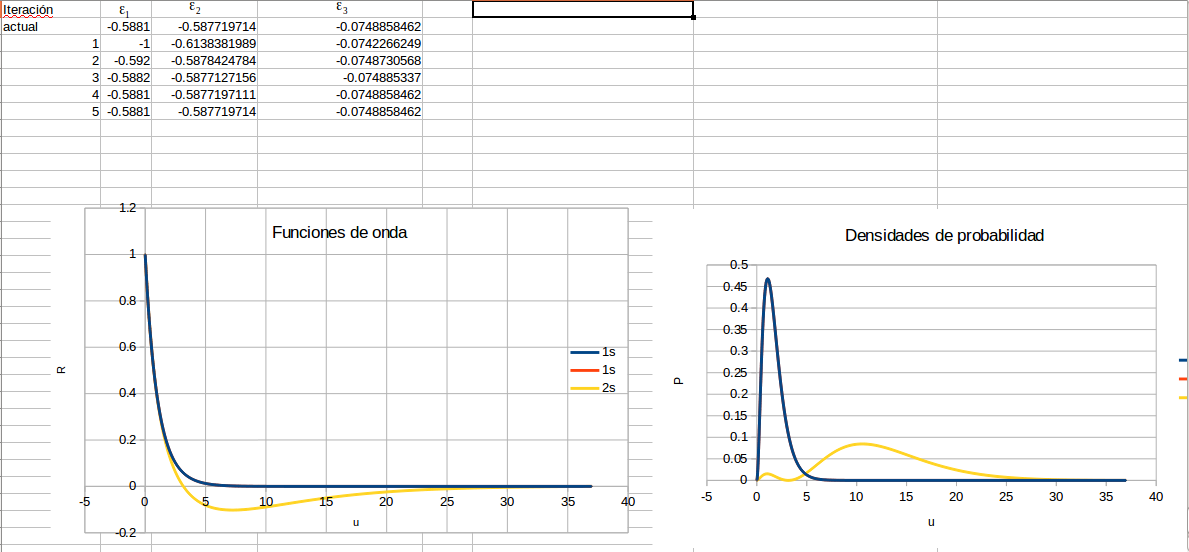
\includegraphics[width = \textwidth]{final_atomica_4.png}
\caption{\label{fig:trabajo}En este sector se ajustaban las energías mediante la generación de gráficas y la herramienta Goal Seek. Una vez se estaba lo suficientemente cerca a la energía deseada se utilizaba este buscador para asegurarse que la cola de la función de onda fuera menor a $0.0001$.}
\end{center}
\end{figure}

\begin{figure}
\begin{center}
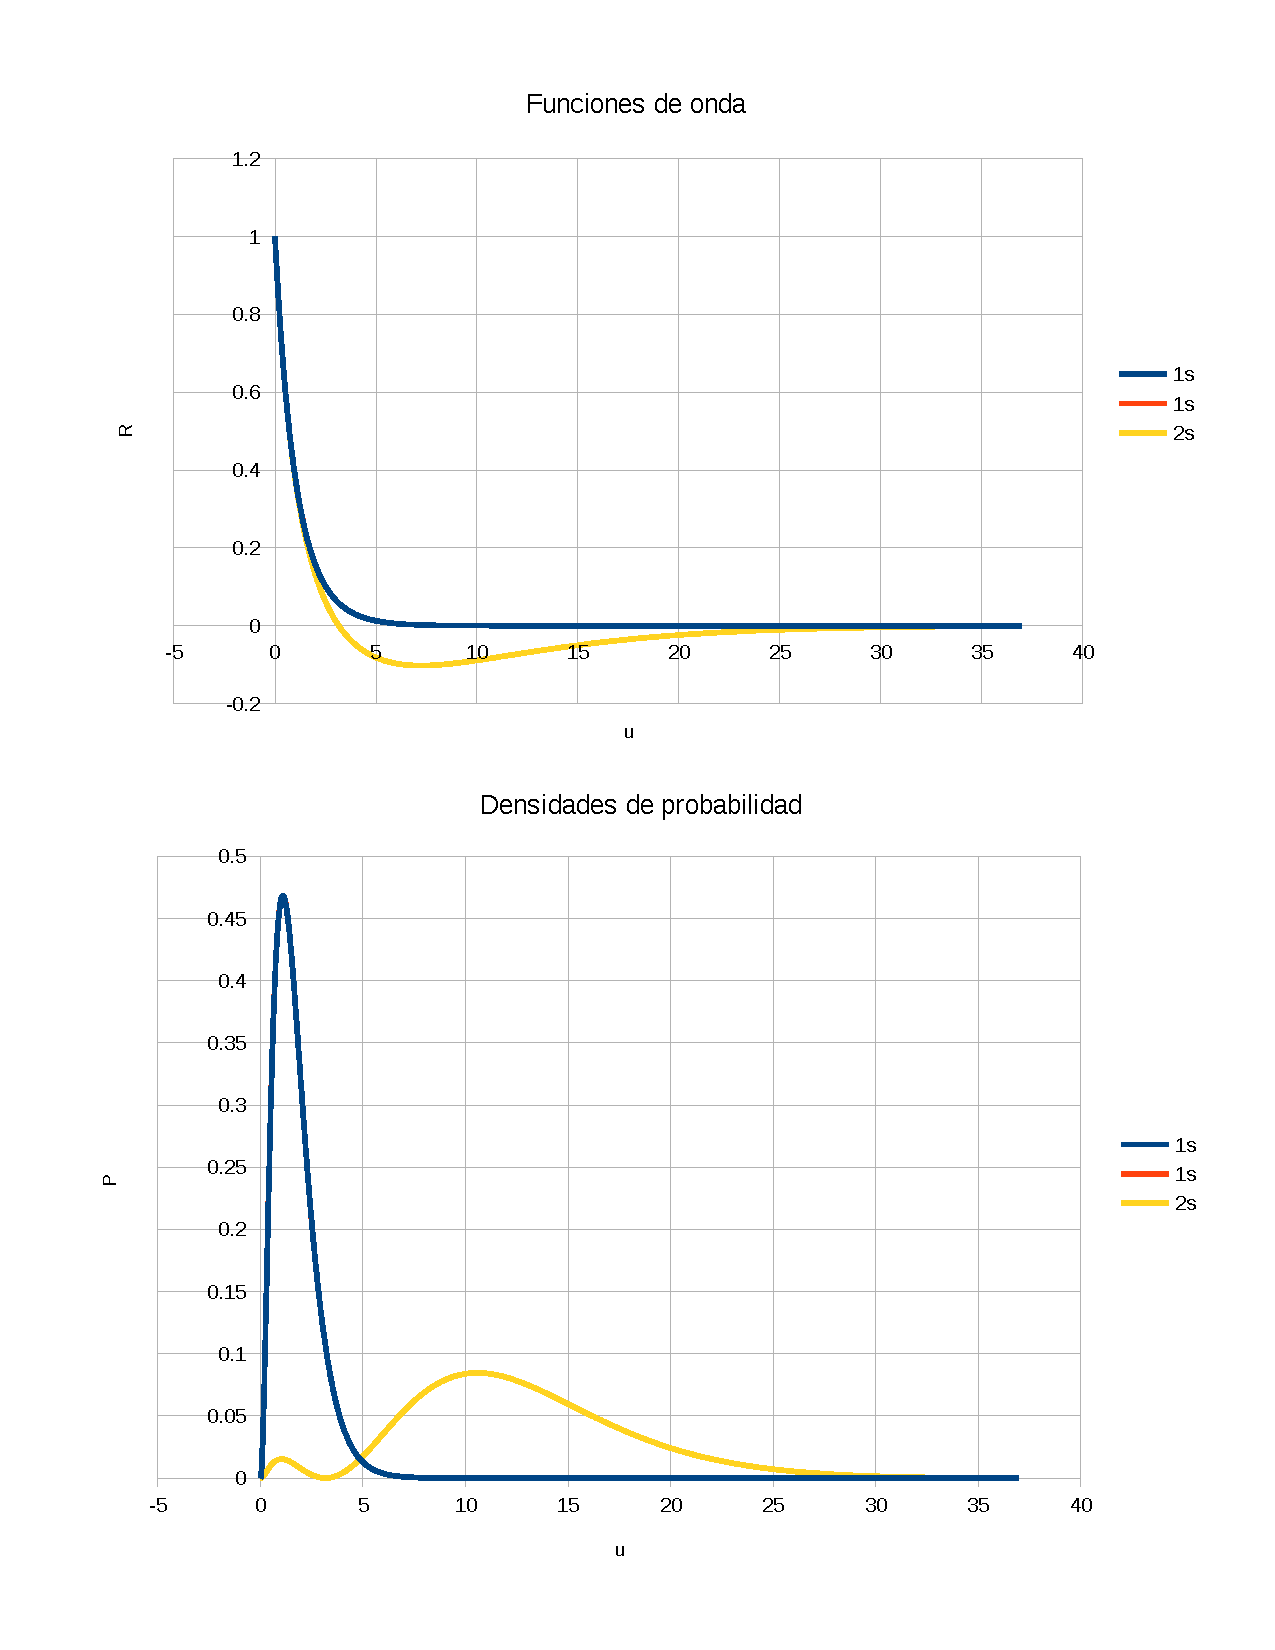
\includegraphics[width = \textwidth]{1s_1s_2s.pdf}
\caption{\label{fig:2s}Se muestran las funciones de onda y las distribuciones de probabilidad asociadas a la configuración $1s^22s$. Se realizaron 5 iteraciones que entregaron finalmente las energías $-0.588$, $-0.588$ y $-0.0749$ para una energía total de $-1.251$, es decir, $-153.1eV$}
\end{center}
\end{figure}

\begin{figure}
\begin{center}
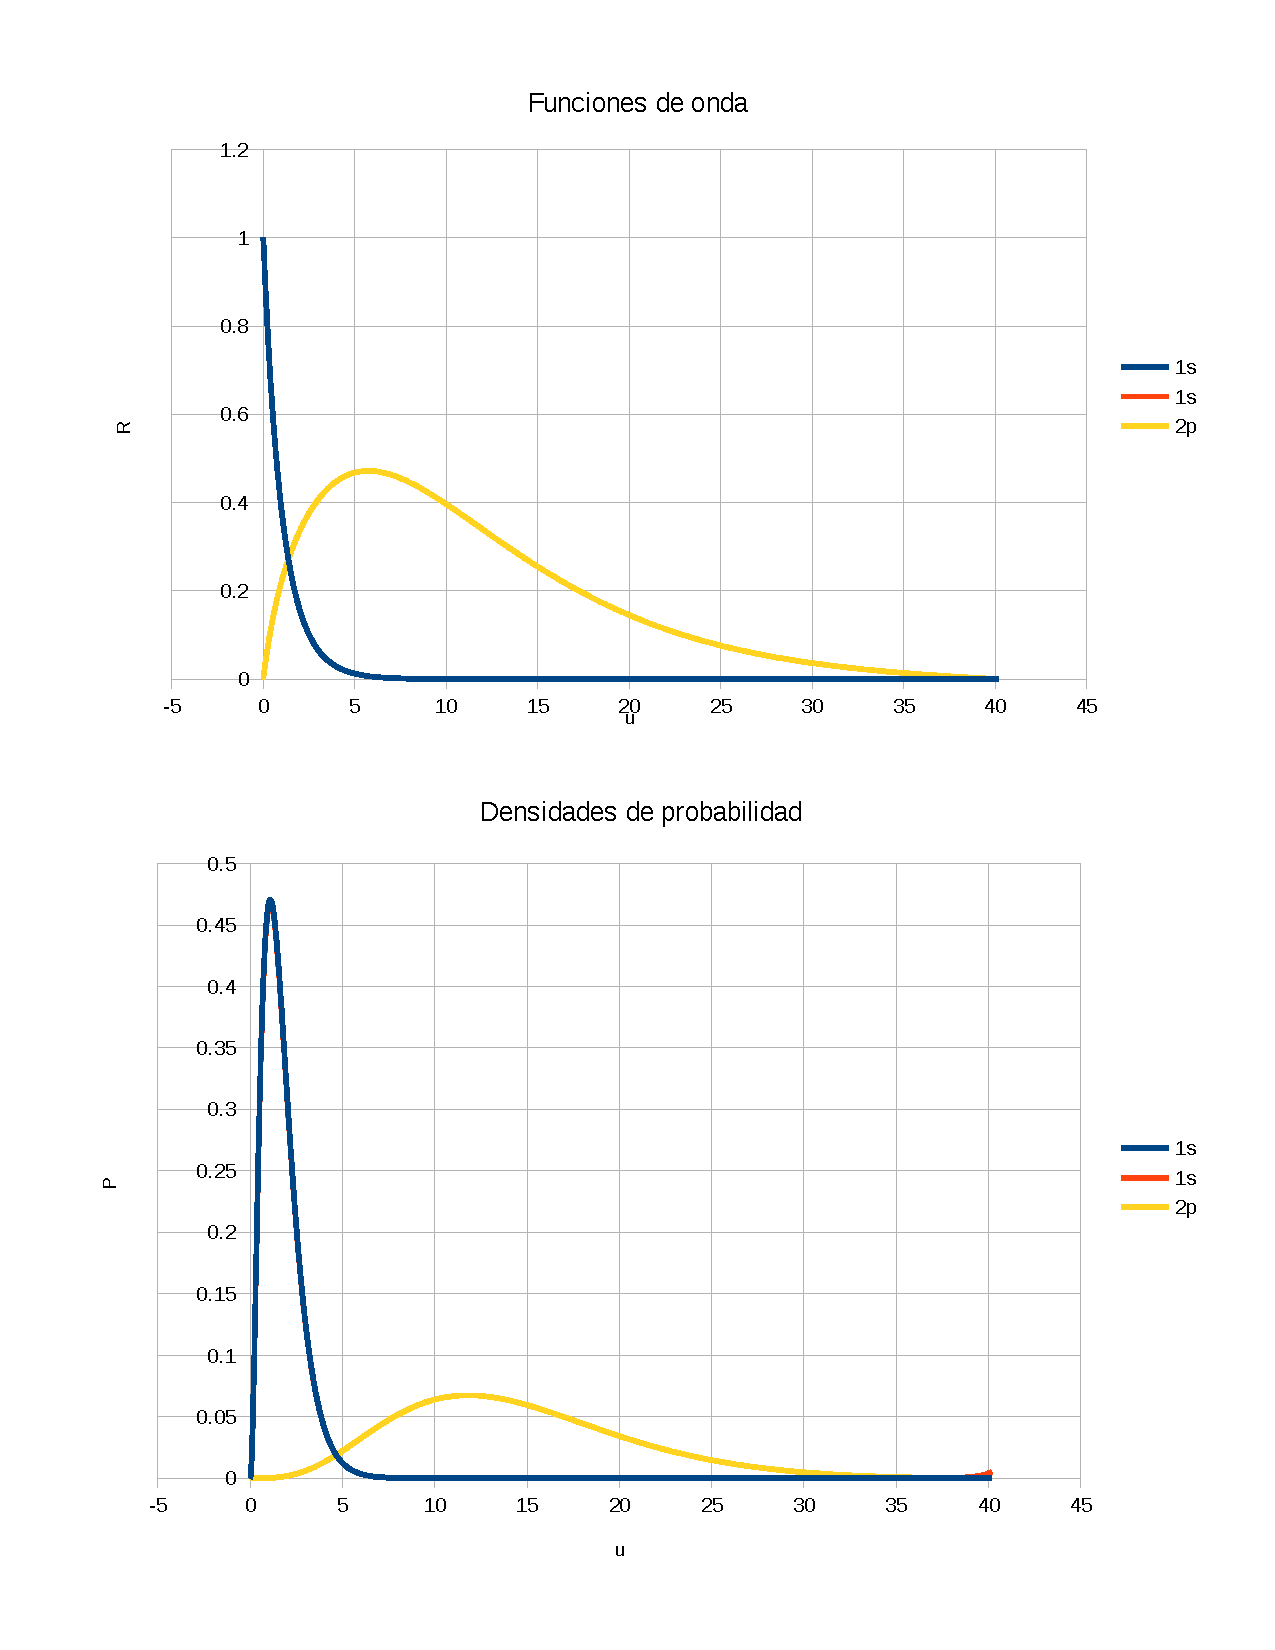
\includegraphics[width = \textwidth]{1s_1s_2p.pdf}
\caption{\label{fig:2p}Se muestran las funciones de onda y las distribuciones de probabilidad asociadas a la configuración $1s^22p$. Se realizaron 3 iteraciones que entregaron finalmente las energías $-0.595$, $-0.595$ y $-0.0609$ para una energía total de $-1.251$, es decir, $-153.1eV$}
\end{center}
\end{figure}

\begin{figure}
\begin{center}
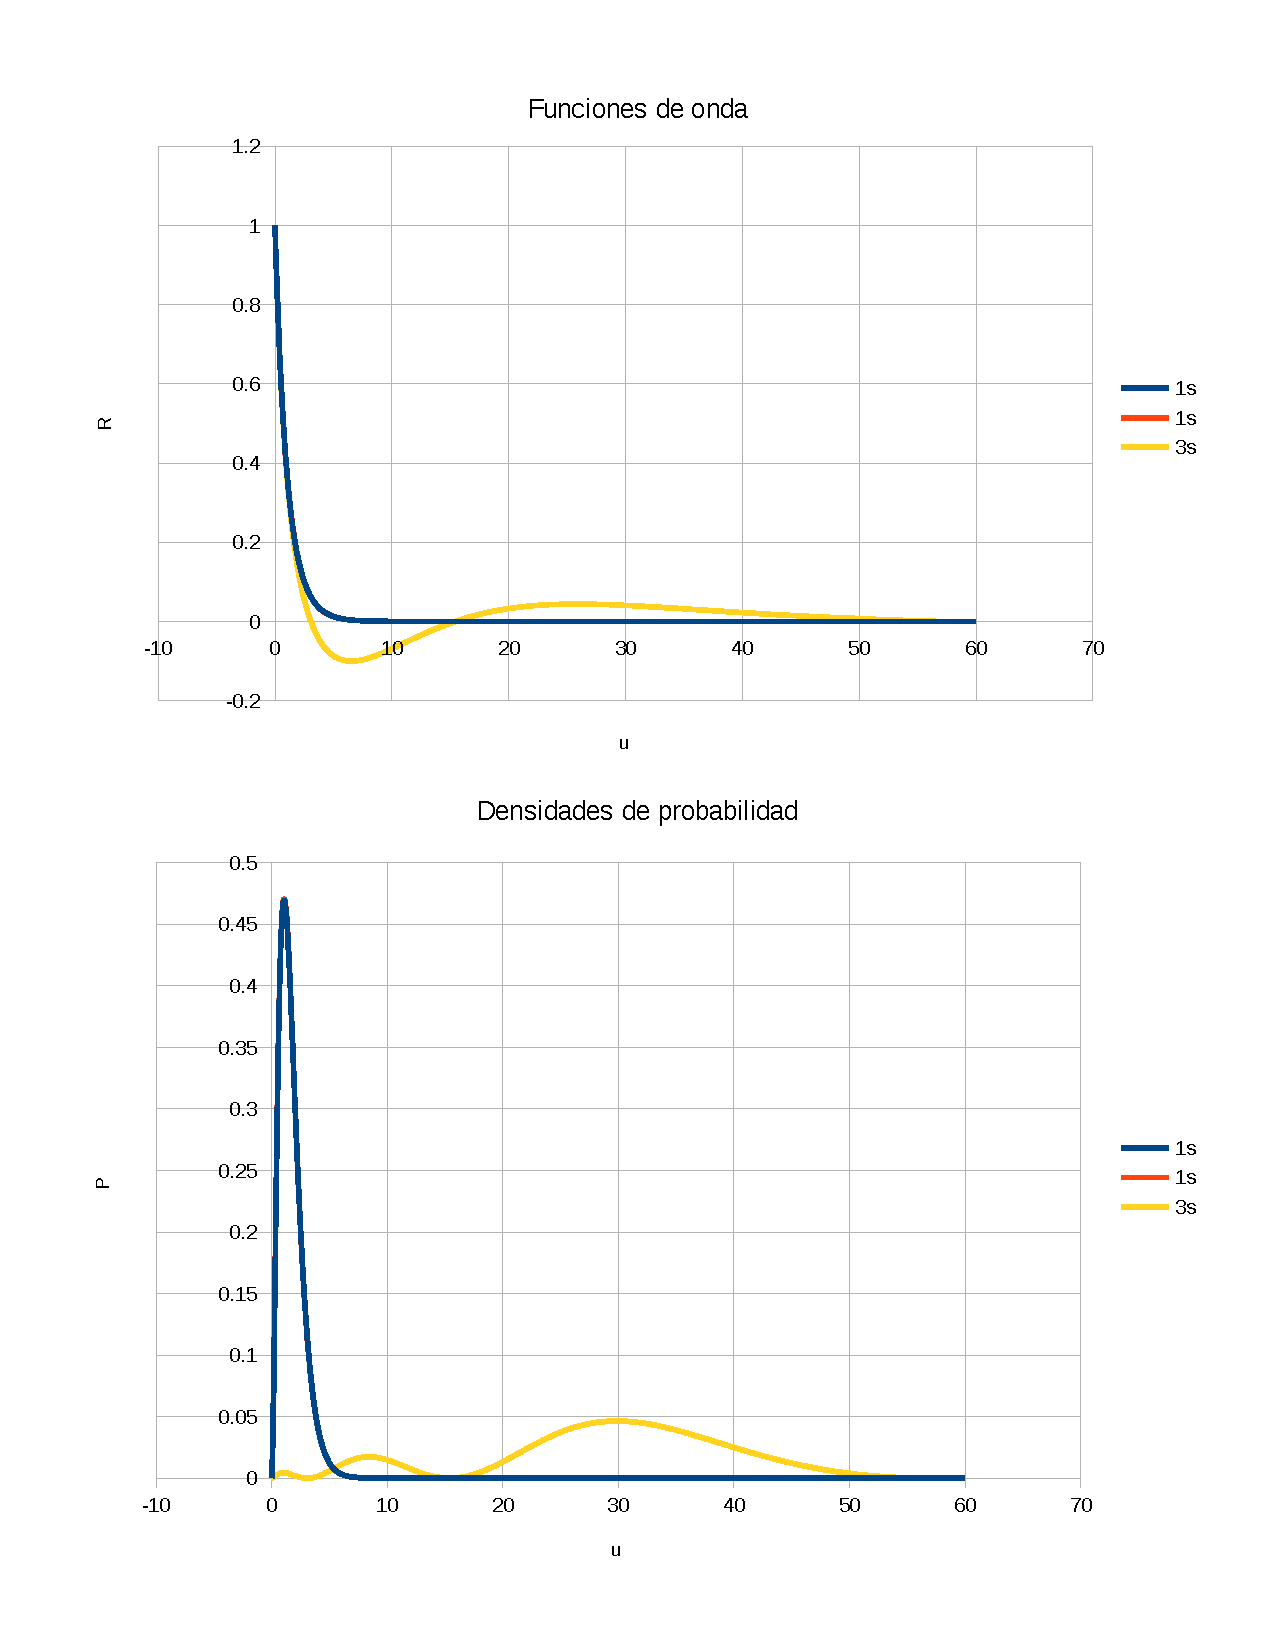
\includegraphics[width = \textwidth]{1s_1s_3s.pdf}
\caption{\label{fig:3s}Se muestran las funciones de onda y las distribuciones de probabilidad asociadas a la configuración $1s^23s$. Se realizaron 5 iteraciones que entregaron finalmente las energías $-0.632$, $-0.633$ y $-0.0592$ para una energía total de $-1.324$, es decir, $-162.0eV$}
\end{center}
\end{figure}

\begin{figure}
\begin{center}
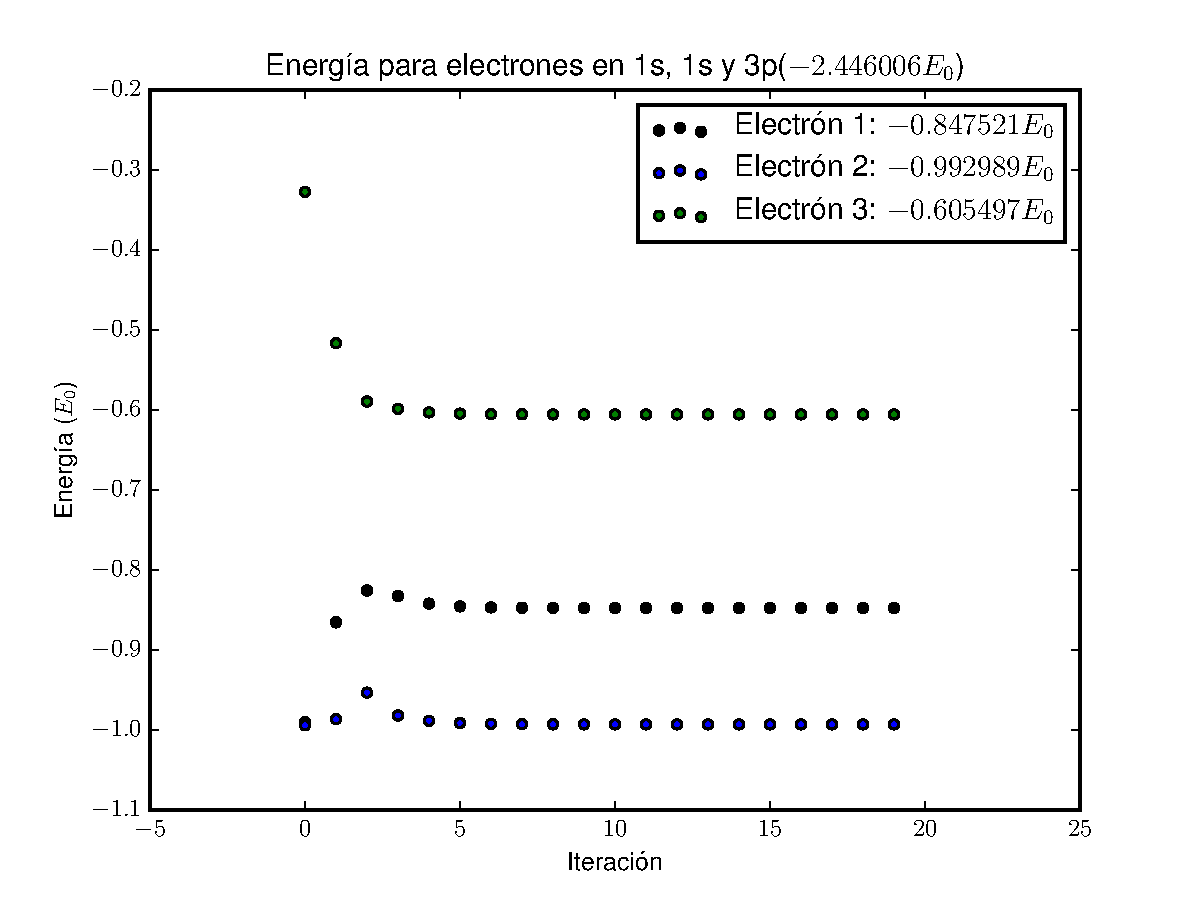
\includegraphics[width = \textwidth]{1s_1s_3p.pdf}
\caption{\label{fig:3p}Se muestran las funciones de onda y las distribuciones de probabilidad asociadas a la configuración $1s^23p$. Se realizaron 3 iteraciones que entregaron finalmente las energías $-0.633$, $-0.635$ y $-0.0560$ para una energía total de $-1.324$, es decir, $-162.0eV$}
\end{center}
\end{figure}

\begin{figure}
\begin{center}
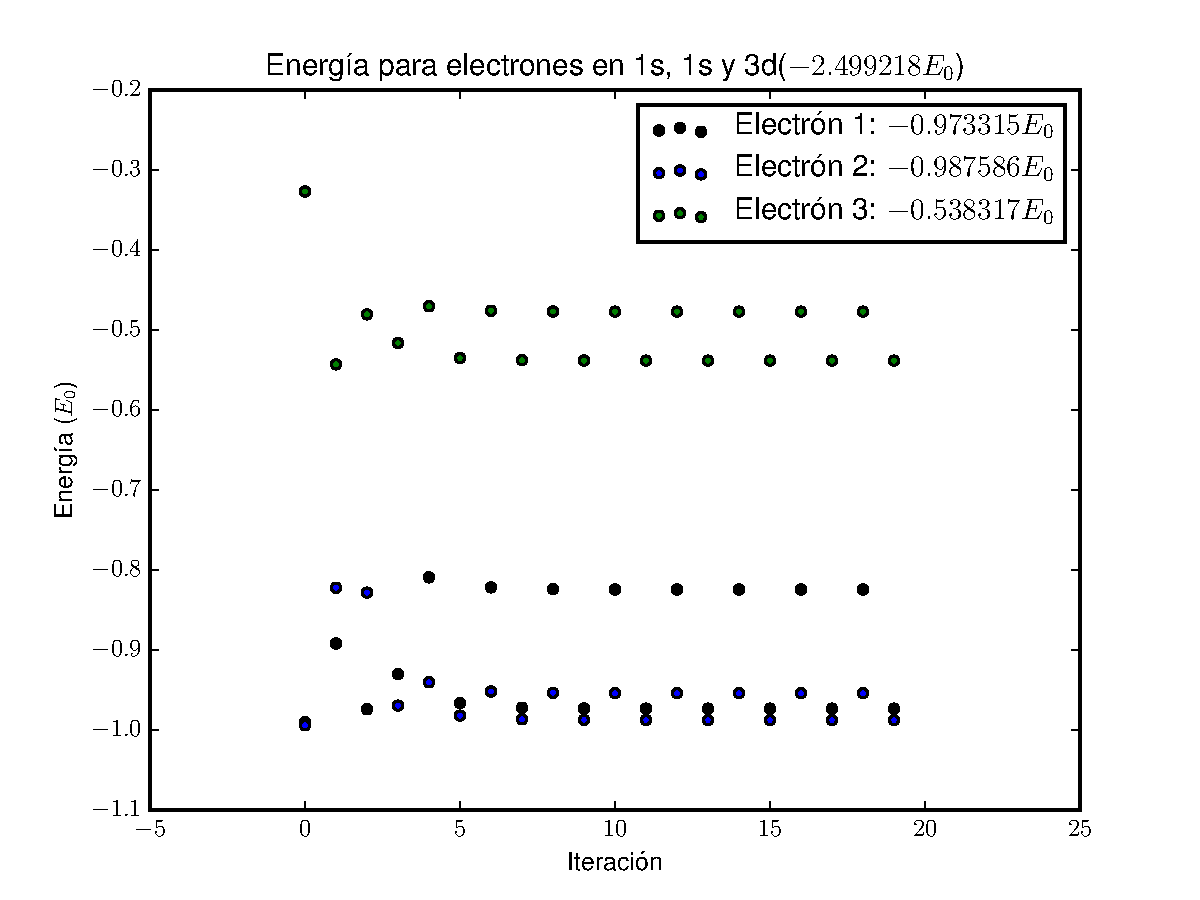
\includegraphics[width = \textwidth]{1s_1s_3d.pdf}
\caption{\label{fig:3d}Se muestran las funciones de onda y las distribuciones de probabilidad asociadas a la configuración $1s^23d$. Se realizaron 3 iteraciones que entregaron finalmente las energías $-0.635$, $-0.637$ y $-0.0563$ para una energía total de $-1.328$, es decir, $-162.6eV$}
\end{center}
\end{figure}

\begin{thebibliography}{1}
\bibitem{nist} Kramida, A., Ralchenko, Yu., Reader, J., and NIST ASD Team (2015). NIST Atomic Spectra Database (ver. 5.3), [Online]. Available: http://physics.nist.gov/asd [2017, May 29]. National Institute of Standards and Technology, Gaithersburg, MD. 
\end{thebibliography}

\end{document}